\documentclass[a4paper]{article}

\usepackage[utf8]{inputenc}
\usepackage{enumerate}
\usepackage{amssymb}
\usepackage{amsfonts}
\usepackage{amsthm}
\usepackage{amsmath}
\usepackage{graphicx}
\usepackage[ruled,vlined]{algorithm2e}

%   New commands
\newcommand{\xt}{$(X_t)$ }
\newcommand{\om}{$\Omega$ }
\renewcommand\qedsymbol{$\blacksquare$}

%       New Environment

\newtheorem{theorem}{Theorem}
\newtheorem{conjecture}{Conjecture}
\newtheorem{propriete}{Property}[subsection]
\newtheorem{proposition}{Proposition}[subsection]
\newtheorem{corollary}{Corollary}
\newtheorem{definition}{Definition}[subsection]
\newtheorem{lemma}{Lemma}
\newtheorem{remarque}{Remark}[subsection]

%       Math definitions

\newcommand{\A}{\mathcal{A}}
\newcommand{\p}{\mathcal{P}}
\newcommand{\q}{\mathcal{Q}}
\renewcommand{\S}{\mathcal{S}}
\newcommand{\x}{\mathcal{X}}
\newcommand{\y}{\mathcal{Y}}
\newcommand{\z}{\mathcal{Z}}



%       Line numberwithin
%\usepackage[left]{lineno}
%\linenumbers


\begin{document}

%\title{Random sampling of lattice polytopes using Markov chains}
\title{Elementary moves on lattice polytopes}
\author{Julien David, Lionel Pournin, Rado Rakotonarivo}
\maketitle

{\small \noindent{\textbf{Abstract.}} A lattice $(d,k)$-polytope is a polytope contained in the hypercube $[0,k]^d$, and whose coordinates of vertices are integers. In order to alter a lattice $(d,k)$-polytope $P$ with vertex set $\mathcal{V}$ in the most elementary way, one may remove a vertex $x$ from $P$, changing $P$ into the convex hull of $\mathcal{V}\mathord{\setminus}\{x\}$. The inverse move consists in inserting a lattice point $x\in[0,k]^d$ as a new vertex of $P$, thus transforming $P$ into the convex hull of $\mathcal{V}\cup\{x\}$, provided $\mathcal{V}\cup\{x\}$
is the vertex set of its convex hull. We show that the graph $\Gamma(d,k)$ whose vertices are the $d$-dimensional lattice $(d,k)$-polytope and whose edges correspond to these elementary moves is always connected. We also prove that the primitive zonotopes introduced by Deza, Manoussakis and Onn are locally maximal in this graph with respect to the number of vertices, for all $d$ and $k$. It follows that the subgraph of $\Gamma(d,k)$ induced by the polytopes with at least $n$ vertices can be disconnected when $n>d+1$. As an application of our connectedness result, we define a Markov chain for the random generation of $d$-dimensional lattice $(d,k)$-polytopes, whose stationary distribution is uniform for all $d\geq2$ and positive $k$.}

\section{Introduction}

Polytopes are convex hulls of finite sets of points in $\mathbb{R}^d$. These objects appear in a wide range of mathematical works, both in theoretical and applied contexts \cite{Ziegler1995}, yet their combinatorics is not well understood. A class of polytopes of special interest in combinatorics is that of \emph{lattice $(d,k)$-polytopes}. These polytopes are contained in the hypercube $[0,k]^d$, where $k$ is a positive integer, and their vertices have integer coordinates. They are a convenient model for the study of any polytope whose vertices have rational coordinates. Lattice polytopes contain a number of very interesting and widely studied classes of polytopes (see for instance \cite{DezaManoussakisOnn2018, GrandeRue2015}). A significant research effort is focusing on evaluating the maximal possible diameter of lattice $(d,k)$-polytopes as a function of $d$ and $k$ \cite{DelPiaMichini2016,DezaManoussakisOnn2018,DezaPournin2018,KleinschmidtOnn1992,Naddef1989}, a problem related to the Hirsch conjecture \cite{BonifasDiSummaEisenbrandHahnleNiemeier2014,BorgwardtDeLoeraFinhold2016,KalaiKleitman1992,KleeWalkup1967,Santos2012} and, more generally, to the complexity of the simplex algorithm.

Yet, the combinatorics of lattice $(d,k)$-polytopes is still barely understood and, as far as we know, there is no result on their structure as a set. In this article, we focus on the latter question. More precisely, we investigate whether it is always possible to connect two lattice $(d,k)$-polytopes by a sequence of lattice $(d,k)$-polytopes such that the vertex sets of two consecutive polytopes in that sequence can be obtained from one another by the insertion or the deletion of a single vertex. Without any other assumption, the problem is trivial since it is always possible to remove the vertices of a polytope one by one and eventually reach the empty polytope. However, if one restricts to the lattice $(d,k)$-polytopes with at least $n$ vertices, where $n$ is a fixed constant, or even simply to the lattice $(d,k)$-polytopes of dimension $d$, the problem turns out to be surprisingly tricky. Consider the graph $\Gamma(d,k)$ whose vertices are the $d$-dimensional lattice $(d,k)$-polytope and whose edges connect two polytopes as soon as the vertex set of one of them is obtained by inserting a lattice point into the vertex set of the other. We will show that the subgraph of $\Gamma(d,k)$ induced by the polytopes with at least $n$ vertices can be disconnected when $n>d+1$, using constructions inspired from the primitive zonotopes recently introduced by Deza, Manoussakis and Onn \cite{DezaManoussakisOnn2018}. In the $2$-dimensional case, we prove the following stronger statement: the subgraph of $\Gamma(d,k)$ induced by the polygons with at least $n$ vertices is disconnected for all $n>3$. However, we will also prove that $\Gamma(d,k)$ itself is connected for all $d\geq2$ and all positive $k$. In other words, full-dimensional simplices make it possible to connect any two lattice $(d,k)$-polytopes within $\Gamma(d,k)$, and they cannot be avoided. Note that the proof of this connectedness result is surprisingly involved, which tells something about how complex lattice $(d,k)$-polytopes are as a set. As an application of this connectedness result, we define a Markov chain that allows to generate $d$-dimensional lattice $(d,k)$-polytopes randomly and prove that the stationary distribution is uniform for all $d\geq2$ and positive $k$.

Consider a lattice $(d,k)$-polytope $P$ with vertex set $\mathcal{V}$. If, for some lattice point $x\in[0,k]^d$, there is a polytope $P'$ with vertex set $\mathcal{V}\cup\{x\}$, we say that $P'$ is obtained from $P$ by an insertion move on $x$ (or simply by inserting $x$). Inversely, we say that $P$ is obtained from $P'$ by a deletion move on $x$ (or, equivalently, by deleting $x$). We show in Section \ref{sec.insert} that, when $d\geq2$ and $k$ is positive, it is possible to perform an insertion move on at least one lattice point from any $d$-dimensional lattice simplex contained in $[0,k]^d$. Building on this result, we prove in Section \ref{sec.conect} that $\Gamma(d,k)$ itself is connected for all $d\geq2$ and $k\geq1$. We also provide in this section examples of lattice polytopes for which no insertion move is possible, and obtain as a consequence that the announced subgraphs of $\Gamma(d,k)$ are disconnected. In section \ref{sec.Markov}, we define our Markov chain and an associated random sampler for $d$-dimensional lattice $(d,k)$-polytopes, and we prove that the stationary distribution of the Markov chain is uniform.

% In order to better understand this class of polytopes, we design a random sampler for them using a Markov chain whose space of states is the set of all $d$-dimensional lattice $(d,k)$-polytopes.
%
%The transitions in this Markov chain, and the resulting random sampler can be described informally as follows. Given a lattice $(d,k)$-polytope $P$ with vertex set $\mathcal{V}$, performing a transition will first consist in randomly choosing a lattice point $x$ in $[0,k]^d$, and then to proceed according to the placement of $x$ with respect to $P$. If $x$ belongs to $\mathcal{V}$, then $P$ will be replaced by the convex hull of $\mathcal{V}\mathord{\setminus}\{x\}$, thus removing $x$ from $P$. If $x$ does not belong to $\mathcal{V}$ and $\mathcal{V}\cup\{x\}$ is precisely the vertex set of its convex hull, then $P$ will be replaced by the convex hull of $\mathcal{V}\cup\{x\}$, thus inserting $x$ in $P$. If none of these two cases occurs, then $P$ will not be affected. A formal definition of this Markov chain shall be given in Section \ref{Sec.MC}. In this article we provide both theoretical and experimental results regarding the behaviour of this Markov chain. Our main result is that the resulting random sampler for lattice $(d, k)$-polytopes is uniform. This is shown in Section \ref{Sec.Pr}. Section X  concludes the article with a number of experiments on the mixing time of our Markov chain.

\section{The insertion move for lattice simplices}\label{sec.insert}

Consider a $d$-dimensional lattice simplex $S$ contained in $[0,k]^d$, where $d\geq2$ and $k\geq1$. Let $\mathcal{V}$ be the set of vertices of $S$. For any vertex $u\in\mathcal{V}$, denote by $H_u$ the affine hull of the facet of $\S$ opposite $u$, and by $H_u^-$ the closed half-space of $\mathbb{R}^d$ limited by $H_u$ that does not contain $u$.
For any $v\in\mathcal{V}$, the intersection
\begin{equation}
  C_v=\bigcap_{\substack{u\in\mathcal{V}\\u\neq{v}}}H_u^-
\end{equation}
is a $d$-dimensional cone pointed at $v$. This cone is exactly the set of the points $x\in\mathbb{R}^d$ such that the convex hull of $S\cup\{x\}$ does not admit $v$ as a vertex. By this remark, we have the following lemma.

\begin{lemma}\label{Lem.A}
Let $x$ be a lattice point in $[0,k]^d$. The convex hull of $S\cup\{x\}$ admits $\mathcal{V}\cup{x}$ as its vertex set if and only if $x$ does not belong to $S$ and, for every vertex $v\in\mathcal{V}$, $x$ does not belong to $C_v$.
\end{lemma}

For any $i\in\{1, ..., d\}$, call
$$
\gamma_i^-=\min\{x_i:x\in{S}\}\mbox{ and }\gamma_i^+=\min\{x_i:x\in{S}\}\mbox{.}
$$

Note that, for all $i\in\{1, ..., d\}$, $\gamma_i^-<\gamma_i^+$ because $S$ is $d$-dimensional. The following is the smallest $d$-dimensional combinatorial hypercube containing $S$, whose facets are parallel to the facets of $[0,k]^d$:
$$
Q=\prod_{i=1}^d[\gamma_i^-,\gamma_i^+]
$$

Consider a facet $R$ of $Q$. The intersection of $R$ and $S$ is a non-empty, proper face $F$ of $S$. Since $S$ is a simplex, it admits another non-empty face $F^\star$ whose vertices are exactly the vertices of $S$ that do not belong to $F$.

By construction,
$$
\mathrm{dim}(F)+\mathrm{dim}(F^\star)=d-1\mbox{.}
$$

In particular, there exists a vector $c$ that is orthogonal to both $F$ and $F^\star$. Consider the hyperplane $Y$ of $\mathbb{R}^d$ that admits $c$ as a normal vector and such that $F^\star\subset{Y}$. The intersection $S\cap{Y}$ is precisely $F^\star$. Denote by $Y^-$ the closed half-space of $\mathbb{R}^d$ bounded by $Y$ that does not contain $F$. In the statement of the following lemma, $\mathrm{aff}(F)$ denotes the affine hull of $F$.

\begin{lemma}\label{Lem.B}
Consider a vertex $v$ of $S$.
\begin{itemize}
\item[i.] If $v$ is a vertex of $F$, then $C_v\cap{Q}$ is a subset of $\mathrm{aff}(F)$,
\item[ii.] If $v$ is a vertex of $F^\star$, then $C_v$ is a subset of $Y^-$.
\end{itemize}
\end{lemma}

\begin{proof}
First observe that, if $s$ is a face of $S$ and $H$ is a hyperplane of $\mathbb{R}^d$ that intersects $S$ exactly along $s$, then
$$
\bigcap_{\substack{u\in\mathcal{V}\\u\not\in{s}}}H_u^-\subset{H^-}\mbox{,}
$$
where $H^-$ is the closed half space of $\mathbb{R}^d$ bounded by $H$ and disjoint from the interior of $S$. Further observe that the intersection of $H$ with
$$
\bigcap_{\substack{u\in\mathcal{V}\\u\not\in{s}}}H_u^-
$$
is precisely the affine hull of $s$. Taking $s=F$ and $H=\mathrm{aff}(R)$, one obtains that for any vertex $v$ of $F$, $C_v\cap{Q}$ is a subset of $\mathrm{aff}(F)$. Taking $s=F^\star$, and $H=Y$, ones obtains that, for any vertex $v$ of $F^\star$, $C_v$ is a subset of $Y^-$.% The result therefore holds because any vertex of $\S$ is either a vertex of $F$ or a vertex of $F^\star$.
\end{proof}

As an immediate consequence of this and Lemma \ref{Lem.A}, for any lattice point $x\in[0,k]^d$ that does not belong to the affine hull of $F$, or to $Y^-$, the convex hull of $S\cup\{x\}$ admits, as vertices, $x$ and all the vertices of $S$.

Assume, without loss of generality that $c$ has norm $1$ and that it points towards $Y^-$. Observe that the intersection of $[0,k]^d$ with the affine hull of $R$ is a $(d-1)$-dimensional cube. Denote
\begin{equation}\label{eq.A}
\delta=\min\{c\mathord{\cdot}x:x\in\mathrm{aff}(R)\cap[0,k]^d\}\mbox{.}
\end{equation}

The set
$$
G=\{x\in\mathrm{aff}(R)\cap[0,k]^d:c\mathord{\cdot}x=\delta\}
$$
is a face of $\mathrm{aff}(R)\cap[0,k]^d$. It follows that $G$ is a cube of dimension at most $d-1$. Recall that $c$ is orthogonal to both $F$ and $F^\star$. As a consequence, the map $x\mapsto{c\mathord{\cdot}x}$ is constant within $F$ and within $F^\star$. Call $\varepsilon$ the value of $c\mathord{\cdot}x$ when $x\in{F}$ and $\varepsilon^\star$ the value of $c\mathord{\cdot}x$ when $x\in{F^\star}$. Since $F$ and $Y^-$ are disjoint, $\varepsilon<\varepsilon^\star$. Moreover, by (\ref{eq.A}), $\delta\leq\varepsilon$. Observe that the latter inequality is strict if and only if $F$ is not a subset of $G$. In this case, $F$, $G$, and $Y$ belong to distinct parallel hyperplanes and we immediately obtain the following.
\begin{lemma}\label{Lem.BC}
If $F\not\subset{G}$ then $G$ is disjoint from both $\mathrm{aff}(F)$ and $Y^-$.
\end{lemma}

If, on the contrary, $\delta$ and $\varepsilon$ coincide, then $F\subset{G}$. This situation is familiar: we are looking at a lattice simplex $F$ contained in a (possibly degenerate) lattice cube $G$. If the dimension of $G$ is greater than the dimension of $F$, then the following lemma provides the desired result.

\begin{lemma}\label{Lem.C}
If $k$ and $d$ are positive and if $P$ is a lattice $(d,k)$-polytope of dimension less than $d$ then there exists a lattice point $x$ that belongs to $[0,k]^d$ but that does not belong to the affine hull of $P$.
\end{lemma}
\begin{proof}
If $P$ is a lattice $(d,k)$-polytope of dimension less than $d$, then the intersection $I$ of its affine hull with $[0,k]^d$ cannot contain more than $(k+1)^{d-1}$ lattice points. Indeed, one can always project $I$ orthogonally on a facet of $[0,k]^d$ in such a way that the dimension of the projection is not less than that of $I$. Such a projection induces an injection from the lattice points in $I$ into the lattice points in the facet on which the projection is made.

Now observe that $[0,k]^d$ contains $(k+1)^d$ lattice points. Since $k$ is positive, $(k+1)^{d-1}<(k+1)^d$ and the lemma is proven.
\end{proof}

We now have to address the case when, regardless of which facet $R$ of $Q$ is chosen, $F$ is a subset of $G$ and these polytopes have the same dimension.

\begin{lemma}\label{Lem.EA}
Call $g$ the maximal dimension of $F$ over all the possible choices of the facet $R$ among the facets of $Q$. Assume that, for any choice of $R$ among the facets of $Q$, $G$ admits $F$ as a subset and the dimensions of $F$ and $G$ coincide. If the difference $d-g$ is not less than $2$, then for some choice of $R$ such that $F$ has dimension $g$, there exists a lattice point in $R\mathord{\setminus}[\mathrm{aff}(F)\cup{Y^-}]$.
\end{lemma}
\begin{proof}
Consider a facet $R$ of $Q$ such that $F$ has dimension exactly $g$. As $G$ admits $F$ as a subset, $G$ must be a face of $Q$. By the maximality of $g$, the intersection of $S$ with any facet of $Q$ incident to $G$ is precisely $F$. In other words, $G$, $F$, $F^\star$, $Y$, and $c$ do not depend on which facet $R$ of $Q$ is chosen, provided this facet is incident to $G$. As a consequence, and taking advantage of the symmetries of the cube, one can choose $R$ in such a way that all the coordinates of $c$ are non-negative, the largest coordinate of $c$ is $c_1$, and
$$
R=\{x\in{Q}:x_1=\gamma_1^-\}\mbox{.}
$$

Recall that $F^\star$ is non-empty and consider a vertex $v$ of $F^\star$. By the definition of $\varepsilon^\star$, we have:
$$
\sum_{i=1}^dc_iv_i=\varepsilon^\star\mbox{.}
$$

This equality can be transformed into
$$
c_1\gamma_1^-+\sum_{i=2}^dc_iv_i=\varepsilon^\star-c_1(v_1-\gamma_1^-)\mbox{.}
$$

In other words, the orthogonal projection $w$ of $v$ on $R$ (whose coordinates coincide with the coordinates of $v$, except for the first coordinate that is equal to $\gamma_1^-$ instead of $v_1$) satisfies $c\mathord{\cdot}w=\varepsilon^\star-c_1(v_1-\gamma_1^-)$. As $c_1$ is non-zero and as $v_1>\gamma_1^-$, we obtain $c\mathord{\cdot}w<\varepsilon^\star$. It immediately follows that $w\not\in{Y^-}$. Now assume that $d-g$ is at least $2$. In this case, $G$ is the intersection of at least two facets of $Q$. Since $v$ does not belong to any of the facets of $Q$ that contain $G$, then $w$ cannot belong to $G$. As a consequence $w$ does not belong to the affine hull of $F$. By construction, $w$ is a lattice point, and the lemma is proven.
\end{proof}

\begin{theorem}\label{thm.add}
Call $g$ the maximal dimension of $F$ over all the possible choices of the facet $R$ among the facets of $Q$. If $d-g$ is not less than $2$, then one can choose the facet $R$ among the facets of $Q$ in such a way that $F$ has dimension $g$ and, for some lattice point $x$ in $R$, the convex hull of $S\cup\{x\}$ admits $\mathcal{V}\cup\{x\}$ as its vertex set, and the convex hull of $F\cup\{x\}$ is a simplex.
\end{theorem}

\begin{proof}
Assume that $g$ is at most $d-2$. If $R$ can be chosen among the facets of $Q$ in such a way that $F\not\subset{G}$, then let $R$ be any such facet and $x$ a lattice point in $G$. By Lemma \ref{Lem.BC}, $x$ cannot belong to the affine hull of $F$. In particular, the convex hull of $F\cup\{x\}$ is a simplex. Moreover, $x$ does not belong to $Y^-$ either. Hence, by Lemmas \ref{Lem.A}, and \ref{Lem.B}, the convex hull of $S\cup\{x\}$ admits $\mathcal{V}\cup\{x\}$ as its vertex set.

Now assume that for any choice of $R$ among the facets of $Q$, $F\subset{G}$ but $R$ can be chosen such that the dimension of $F$ is less than the dimension of $G$. In this case, by Lemma \ref{Lem.C}, there exists a lattice point $x$ in $G$ that does not belong to the affine hull of $F$. In particular, the convex hull of $F\cup\{x\}$ is a simplex. As in addition, $Y^-$ is disjoint from $G$, it follows from Lemmas \ref{Lem.A}, and \ref{Lem.B} that the convex hull of $S\cup\{x\}$ admits $\mathcal{V}\cup\{x\}$ as its vertex set.

Finally, assume that for any choice of $R$ among the facets of $Q$, $F$ is a subset of $G$ and the dimensions of $F$ and $G$ coincide. By Lemma \ref{Lem.EA}, one can choose $R$ such that $F$ has dimension $g$ and there exists a lattice point in $R$ that does not belong to the affine hull of $F$ or to $Y^-$. In this case, the convex hull of $F\cup\{x\}$ is a simplex and, by Lemmas \ref{Lem.A}, and \ref{Lem.B}, the convex hull of $S\cup\{x\}$ admits $\mathcal{V}\cup\{x\}$ as its vertex set, which completes the proof.
\end{proof}

The following corollary shows that an insertion move is possible for $S$ on at least one lattice point. The argument in this proof will be used again in the next section, in order to prove that $\Gamma(d,k)$ is always connected.

\begin{corollary}\label{cor.add}
There exists a lattice point $x$ in $[0,k]^d$ such that the convex hull of $S\cup\{x\}$ admits $\mathcal{V}\cup\{x\}$ as its vertex set.
\end{corollary}
\begin{proof}
If, for any possible choice of $R$ among the facets of $Q$, the dimension of $F$ is at most $d-2$, then the result follows from Theorem \ref{thm.add}. Assume that, for some facet $R$ of $Q$, $F$ has dimension $d-1$. In this case, $Y$ is parallel to $R$ and $F^\star$ is made up of a single vertex, say $v$. By the same argument as in the proof of Lemma \ref{Lem.B}, the intersection of $C_v$ with $Y$ is precisely $v$ and, for every vertex $u$ of $F$, $C_u$ is disjoint from $Y$. Hence, by Lemma \ref{Lem.A}, any lattice point $x$ in $Y\cap[0,k]^d$ distinct from $v$ is such that the convex hull of $S\cup\{x\}$ admits $\mathcal{V}\cup\{x\}$ as its vertex set. As $k\geq1$, there exists at least one such lattice point.
\end{proof}

\section{The connectivity of $\Gamma(d,k)$}\label{sec.conect}

We first prove in this section that $\Gamma(2,k)$ is a connected graph. This will serve as the base case for the inductive proof that $\Gamma(d,k)$ is connected. In the whole section, we call \emph{corner simplex} of $[0,k]^d$ the simplex whose vertices are the origin (the lattice point whose all coordinates are zero), and the $d$ lattice points in $[0,k]^d$ distant from the origin by exactly $1$.

\begin{theorem}\label{thm.Connec2}
For any positive $k$, $\Gamma(2,k)$ is connected.
\end{theorem}
\begin{proof}
Consider a lattice polygon $P$ contained in the square $[0,k]^2$. First observe that, if $P$ is not a simplex, then a deletion move can always be performed for some vertex of $P$. In particular, $P$ can always be transformed into a lattice triangle by a sequence of deletions. Hence, in order to prove the theorem, we only need to show the connectedness of the subgraph of $\Gamma(2,k)$ induced by triangles and quadrilaterals. Consider a lattice triangle contained in the square $[0,k]^2$. If this triangle does not have a horizontal or a vertical edge then, by Theorem \ref{thm.add}, an insertion move can be performed to transform it into a quadrilateral with a horizontal or a vertical edge, say $e$. It is then possible to perform a deletion move on one of the vertex of  this quadrilateral that is not incident to $e$ in order to obtain a triangle $T$ that admits $e$ as an edge. The strategy is then to transform $T$ into the corner triangle of $[0,k]^2$ using the sequence of moves sketched in Fig. \ref{fig:connect}. This figure shows the case when $e$ is the horizontal edge on the bottom of $T$. In each portion of the figure, the next point on which a move will be performed is colored blue. First observe that an insertion move can be performed on a lattice point in the line parallel to $e$ that contains the vertex of $T$ opposite $e$ in order to obtain a quadrilateral with three horizontal or vertical edges as shown in Figs. \ref{fig:connect}(i) and \ref{fig:connect}(ii).
\begin{figure}[b]
\begin{center}
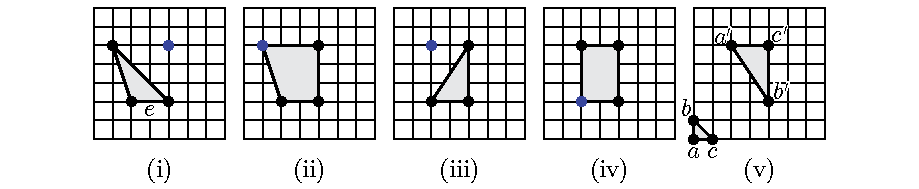
\includegraphics[width=\textwidth]{assets/connect}
\caption{An illustration of the sequence of deletion and insertion moves from the lattice triangle in (i) to the corner triangle on the bottom-left of (v).}
\label{fig:connect}
\end{center}
\end{figure}
A deletion move on one of the vertices of the quadrilateral then results in a triangle with a horizontal and a vertical edge shown in Fig. \ref{fig:connect}(iii). After that, the triangle has a unique oblique edge that faces one of the four vertices of the square $[0,k]^2$. It is always possible to make this edge face the vertex on the bottom left of the square by performing an insertion move to obtain a rectangle and then a deletion move on the bottom-left vertex of the rectangle. This sequence of moves is illustrated in Figs. \ref{fig:connect}(iii) and \ref{fig:connect}(iv) in the case when the oblique edge initially faces the top left vertex. Finally, one can transform the resulting triangle into the corner triangle of $[0,k]^2$ by inserting the vertices labeled $a$, $b$, and $c$ in Fig. \ref{fig:connect}(v) in this order, the insertion of $x$ being immediately followed by the deletion of $x'$.
\end{proof}

\begin{theorem}\label{lem.Connecd}
For any $d\geq2$ and any positive $k$, $\Gamma(d,k)$ is connected.
\end{theorem}
\begin{proof}
The proof proceeds by induction on $d$. The base case is provided by Theorem \ref{thm.Connec2}. Again, one can always transform a $d$-dimensional lattice $(d,k)$ polytope into a $d$-dimensional simplex by a sequence of deletion moves. Therefore, we only need to prove that the subgraph induced in $\Gamma(d,k)$ by simplices and by polytopes with $d+2$ vertices is connected. The strategy will be, again, to transform any simplex in this graph into the corner simplex of $[0,k]^d$.

Assume that $d\geq3$, consider a lattice simplex $S$ contained in $[0,k]^d$, and call $\mathcal{V}$ the vertex set of $S$. For any $i\in\{1, ..., d\}$, call
$$
\gamma_i^-=\min\{x_i:x\in{S}\}\mbox{ and }\gamma_i^+=\min\{x_i:x\in{S}\}\mbox{.}
$$

Further denote
$$
Q=\prod_{i=1}^d[\gamma_i^-,\gamma_i^+]\mbox{.}
$$

Call $g$ the maximal dimension of the intersection of $S$ and a facet of $Q$. If $g$ is at most $d-2$ then, by Theorem \ref{thm.add}, there exists a facet $R$ of $Q$ such that $S\cap{R}$ is $g$-dimensional and a lattice point $x\in{R}$ such that the convex hull of $S\cup\{x\}$ admits $\mathcal{V}\cup\{x\}$ as its vertex set and the convex hull of $[S\cap{R}]\cup\{x\}$ is a simplex. In other words, one can perform an insertion move on vertex $x$ to transform $S$ into a polytope with vertex set $\mathcal{V}\cup\{x\}$. Since the convex hull of $S\cup\{x\}$ is a simplex, one can find a simplex whose vertex set contains all the vertices of $S\cup\{x\}$, and is a subset of $\mathcal{V}\cup\{x\}$. This simplex can be obtained from the convex hull of $\mathcal{V}\cup\{x\}$ by a single deletion move. Now observe that the intersection of this simplex with $R$ has dimension $g+1$. Repeating this procedure provides a sequence of insertion and deletion moves that transform $S$ into a lattice simplex whose intersection $F$ with a facet $R$ of $Q$ has dimension $d-1$. Call $v$ the unique vertex of the lattice simplex that does not belong to $R$. In other words, this lattice simplex is a pyramid with apex $v$ over $F$. Observe that, in this case, any sequence of insertion and deletion moves that can be performed for $F$ within the cube $\mathrm{aff}(R)\cap[0,k]^d$ can also be performed within $[0,k]^d$ for the pyramid with apex $v$ over $F$. By induction, one can transform $F$ into any lattice simplex in $\mathrm{aff}(R)\cap[0,k]^d$ by a sequence of deletion and insertion moves. Therefore, we can build a sequence of moves that transform $S$ into the $d$-dimensional lattice simplex $S'$ whose vertex set is made up of $v$, of the lattice point $w$ in $\mathrm{aff}(R)\cap[0,k]^d$ with a unique non-zero coordinate, and of the $d-1$ lattice points in $\mathrm{aff}(R)\cap[0,k]^d$ distant by exactly $1$ from $w$.

Now observe that one can perform an insertion move on any lattice vertex distinct from $v$ in the intersection of $[0,k]^d$ with the hyperplane parallel to $R$ that contains $v$. We proceed by inserting the lattice point in this intersection whose orthogonal projection on $R$ is $w$ and then, by deleting $v$. Calling $v'$ any of the $d-1$ lattice points in $\mathrm{aff}(R)\cap[0,k]^d$ distant from $w$ by exactly $1$, the simplex that results from the latter deletion is a pyramid with apex $v'$ over a $(d-1)$-dimensional simplex $F'$ such that, for some $i\in\{1, ..., d\}$, $v'$ satisfies $v'_i=1$ and every vertex $u$ of $F'$ satisfies $u_i=0$. Call $R'$ the facet of $[0,k]^d$ made up of the points $x$ such that $x_i=0$. By induction, one can transform $F'$ within $R'$ into the corner simplex of $R'$. From there, one can perform an insertion move on any lattice vertex distinct from $v'$ in the intersection of $[0,k]^d$ with the hyperplane parallel to $R'$ that contains $v'$. We proceed by inserting the lattice point in this intersection whose orthogonal projection on $R'$ is the origin. Since $v'_i=1$, the $i$-th coordinate of the inserted point is $1$, and its other coordinates are all equal to $0$. Hence, after a last deletion move on $v'$, the resulting simplex is the corner simplex of $[0,k]^d$, as desired.
\end{proof}

\section{A Markov chain for lattice polytopes}\label{sec.Markov}

%Recall that our purpose is to build an uniform random sampler of $(d,k)$-polytopes. Given $d$ and $k$, let us consider the $[0,k]^d$ hypercube. The sampler consists in running a random walk on a Markov chain $(X_t)_{t\geq{0}}$ which space of states $\Omega$ is the set of $(d,k)$-polytopes. The transition matrix $P$ will be described as a set of local rules on our $(d,k)$-polytopes.
% INTERIOR POINT
%In our case we define a point $v$ as an \textbf{interior point} of $\mathcal{P}$ if $v$ is either inside or on the boundary of $\mathcal{P}$ and $v$ is not a vertex of $\mathcal{P}$.

We will consider a Markov chain whose space of states $\Omega$ is the set of all $d$-dimensional lattice $(d,k)$-polytopes, for fixed $d$ and $k$. A priori, the definition of lattice $(d,k)$-polytopes does not requires them to be $d$-dimensional. Some effort will be needed in order to enforce the requirement that all the states of our Markov chain are polytopes of dimension exactly $d$. % Thus we assume that $\p=\{x_1, x_2, …, x_n\}$ means $\p=Conv(\{x_1, x_2, …, x_n\})$, where the $x_i$ are lattice points of $[0,k]^d$. Note that:
%
%\begin{enumerate}
%  \item $\p-\{x_j\}$ is the convex hull in which we had remove exactly the $j-$th vertex of $\p$. We note that $\p-\{v_j\}$ is also a state of $\Omega$, and it is fulldimentional only if $|\p|>d+1$.
%  \item $\p \cup \{v\}$ where $v \in [0,k]^d$, is the convex hull where we add exactly one point without removing any vertices of $\p$. We can observe that
%  $$
%    |Conv(\p \cup \{v\})| = |\p| + 1 \mbox{.}
%  $$
%\end{enumerate}
The transition rules of our Markov chain are defined as local operations on lattice $(d,k)$-polytopes. These rules consist in adding or removing a given vertex to such a polytope. Consider a $d$-dimensional lattice $(d,k)$-polytope $P$ and denote by $\mathcal{V}$ its vertex set. Consider a lattice point $x$ in $[0,k]^d$ which, we assume has been uniformly drawn from all possible lattice points in $[0,k]^d$. The transition from $P$ that corresponds to the chosen lattice point $x$ goes as follows.

\begin{itemize}
\item If $x$ is contained in $P$ but is not a vertex of it (i.e. $x\in{P}\mathord{\setminus}\mathcal{V}$) then the chain will loop on $P$. In other words, the current state is unaffected.
\item If $x$ is a vertex of $P$ (i.e. $x\in\mathcal{V}$), then
  \begin{itemize}
    \item If the convex hull $Q$ of $\mathcal{V}\mathord{\setminus}\{x\}$ is $d$-dimensional, the transition goes from $P$ to $Q$. Note that if $Q$ were $(d-1)$-dimensional, then $P$ would be a pyramid (with apex $x$) over $Q$. In this case, the transition from $P$ to $Q$ would be impossible because it would exit $\Omega$.
    \item Otherwise, we loop on $P$.
  \end{itemize}
  \item If $x$ does not belong to $P$, then
  \begin{itemize}
    \item If $\mathcal{V}\cup\{x\}$ is precisely the vertex set of its convex hull, then the transition goes from $P$ to the convex hull of $\mathcal{V}\cup \{x\}$.
    \item Otherwise we loop on $P$.
  \end{itemize}
\end{itemize}

Figure \ref{fig:boucle} illustrates transition rule in the case of a lattice triangle $P$ contained in the square $[0,4]^2$, depending on the placement of point $x$. Note that in this particular case, there is no transition that deletes a vertex of $P$.
% \begin{figure}
%   \begin{center}
%     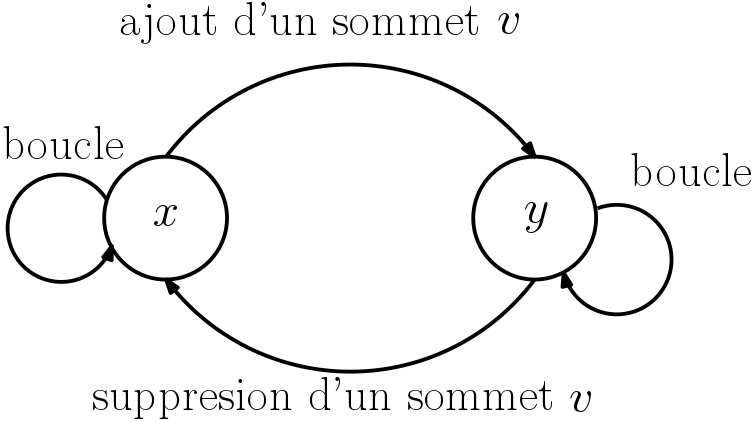
\includegraphics[scale=0.3]{assets/transition}
%     \caption{Transition relation between two states $x$ and $y$ in $\Omega$: either $y = x \cup \{v\}$ and $x = y - \{v\}$ or $v$ has been moved respectivly from $x$ to get $y/$ from $y$ to get $x$, where $v \in [0,k]^d$.}
%     \label{fig:fig2}
%   \end{center}
% \end{figure}

\begin{figure}
  \begin{center}
    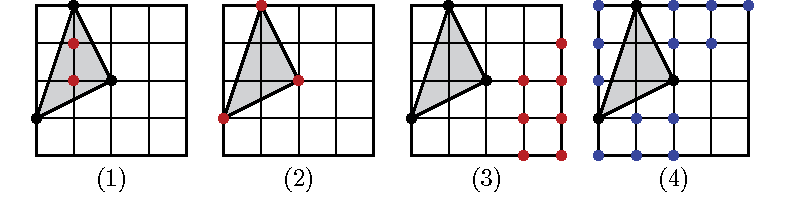
\includegraphics[scale=0.9]{assets/boucle-mod}
    \caption{An illustration of the transition rule for a triangle (depicted in grey), depending on the placement of point $x$, colored red when the chain loops and blue when it does not loop: (1) $x$ belongs to $P\mathord{\setminus}\mathcal{V}$, (2) the convex hull of $\mathcal{V}\mathord{\setminus}\{x\}$ is $(d-1)$-dimensional, (3) $\mathcal{V}\cup\{x\}$ is not the vertex set of its convex hull, and (4) the transition changes $P$ into the convex hull of $\mathcal{V}\cup\{x\}$.}
    \label{fig:boucle}
  \end{center}
\end{figure}

\subsection{Irreducibility of $(X_t)$}

\begin{lemma}\label{lem:elim-mauvais-cas}
  For any simplex $x \in \Omega$, for any $y \in \Omega$. If we cannot reduce $x \bigtriangleup y$ by adding a vertex in $y \setminus x$ the there exists a simplex $z \in \Omega$, a transition state between $x$ and $y$, which verifies:
  \begin{itemize}
    \item $|x \bigtriangleup y| = |z \bigtriangleup y|$
    \item $\delta(x,z)\leq{2}$
  \end{itemize}
  such that we can always add a vertex in $y \setminus z$, from $z$ to $y$.
\end{lemma}

\begin{proof}
Let be $x$ a simplex $y$ be in $\Omega$. Let be $v \in [0,k]^d$. The idea of the proof lies on the fact that, $z$ will be found by adding a point $v \in \Omega$ and which is not an element of $x \bigtriangleup y$, then remove a point of $x \setminus y$. In this way we found the simplex $z$ at most in 2 steps.
\end{proof}

\begin{lemma}\label{lem:irreducibility}
  For all $x$ and $y \in \Omega$, there exists $z \in \Omega$ which satisfies $|x \bigtriangleup y| > |z \bigtriangleup y|$ such that $\delta(x,z)\leq{3}$.
\end{lemma}

\begin{proof}
  Let $x$ and $y$ be states of $\Omega$, such that $P(x,y)=0$. Let $z$ be a transition state between $x$ and $y$, and such that $z$ is closer to $y$ than $y$. We have several distinct cases:

  \begin{enumerate}
    \item $x$ is not a simplex.
    \begin{enumerate}
      \item $x \subset y$: add $v \in y \setminus x$ and $z = x \cup \{v\}$, then $\delta(x,z) = 1$
      \item $x \not\subset y$: remove $v \in x \setminus y$ and $z = x - \{v\}$, then $\delta(x,z) = 1$
    \end{enumerate}
    \item $x$ is a simplex.
    \begin{enumerate}
      \item If we can add $v \in y \setminus x$ then add it, thus $z = x \cup \{v\}$ and $\delta(x,z) = 1$
      \item Else:
      \begin{enumerate}
        \item Add a point $u$ which is not in $x \bigtriangleup y$
        \item Remove a point from  $x \setminus y$
        \item Add  a point from $y \setminus x$

        In this last case, one finds $z$ such that $\delta(x,z) = 3$
      \end{enumerate}
    \end{enumerate}
  \end{enumerate}

  Since we had proved we can always add a point which is not contained in $x \bigtriangleup y$ by lemma \ref{lem:elim-mauvais-cas}. It means that wherever in which case we are, one can always find a $z$ which reduces the symetric difference from $z$ to $y$ by one, such that $\delta(x,z) \leq{3}$.

\end{proof}

\begin{corollary}\label{coro:diameter}
  For all $x$ and $y \in \Omega$ one has:
  \begin{equation}
    \delta(x,y) \leq |x| + |y| + 4(d+1)
  \end{equation}
\end{corollary}

\begin{proof}
  This is an immediate consequence of the lemma \ref{lem:irreducibility}. Let $x$ and $y$ be in $\Omega$. Let us now consider two simplices $x^\star$ and $y^\star$ such that $\delta(x,x^\star) = |x| - (d+1)$, and $\delta(y,y^\star) = |y| - (d+1)$. Thus
  $$
    \delta(x,y) \leq{\delta(x,x^\star) + \delta(x^\star,y^\star) + \delta(y,y^\star)}
  $$
  Since $x^\star$ is a simplex, the walk needs at most $3(|x^\star| + |y^\star|) = 3 \times 2(d+1)$ steps to reach $y^\star$ from $x^\star$. Hence
  $$
    \delta(x,y) \leq{|x| - (d+1) + |y| - (d+1) + 6(d+1)} = |x| + |y| + 4(d+1)
  $$
\end{proof}

Observe that corollary \ref{coro:diameter} gives an idea on the upper bound of the diameter of $(X_t)$. We have now settled all we need to prove our main results on the properties of $(X_t)$.

\begin{theorem}\label{thm:diameter}
  Define the diameter $\mathcal{D}$ of a graph with vertex set $\Omega$ to be the maximum distance between two vertices. For $(X_t)$, as defined above, and given $k$ and $d$, one has:
  \begin{equation}
    \mathcal{D}_{X_t} \leq{2ck^{3/4} + 4(d+1)} \quad \mbox{where} \ c>0
  \end{equation}
\end{theorem}

\begin{proof}
  To be done.
\end{proof}

\begin{theorem}\label{thm:main}
  The Markov chain $(X_t)$ is irreductible, aperiodic and has the uniform as stationnary distribution.
\end{theorem}

\begin{proof}
  Three propreties have to be verified, thus this proof will be given in three steps. Let $x$ and $y$ be in $\Omega$.

  \begin{enumerate}[i]
    \item \textit{Irreducibility}
    Irreducibility is a direct consequence of the corollary \ref{coro:diameter}. Let us remind that to prove the irreducibility, one needs to find a $r_0$ such that, for all $x$ and $y \in \Omega$, when $r \geq{r_0}$ then $P^r(x,y)>0$. Thus let us take $r_0 = |x| + |y| + 4(d+1)$.

     \item \textit{Symetry}
     Our transition rules consists in either add or remove a single vertex for two distinct states. Observe that if there is no one step transition from $x$ to $y$ means $P(x,y)=0$. By the trasition rules, necessarily, if $P(x,y)=0$ then $P(y,x)=0$.
     Next, let us prove that if $P(x,y)>0$ and $P(y,x)>0$ then we also have $P(x,y) = P(y,x)$. $P(x,y)>0$ means that we have a one step transition from $x$ to $y$. Only two cases may occur. For $v \in [0,k^d]$ either $y = x - \{v\}$, or $y = x \cup \{v\}$. Considering the first case, the probability to draw $v$ and add it to $x$ is $P(x,y) = \frac{1}{(k+1)^d}$. Similarily, to move from $y$ to $x$, we draw the same $v$ and remove it from $y$ to get $x$ with probability $P(y,x) = \frac{1}{(k+1)^d} = P(x,y)$. We prove the remaining case in an analog reasoning.

     \item \textit{Aperiodicity}
     To prove that $(X_t)$ is aperiodic, one needs to show that each state in $\Omega$ has as period $1$. Since $(X_t)$ is irreductible, property \ref{prop:irr-ap} tells us that all the states of $\Omega$ has the same period. Thus, for all $x, y \in \Omega$, $\mathrm{gcd}(\mathcal{T}(x)) = \mathrm{gcd}(\mathcal{T}(y))$. One needs to find a state $x$ such that t$\mathrm{gcd}(\mathcal{T}(x)) = 1$. Let us take $x$ has a simplex and a point $v \in [0,k]^d$ then consider the cases where we have a loop on $x$:
     either $v$ is an interior point to $x$, or $v$ is drawn outside of $x$ but $|Conv(x \cup \{v\})| \neq |x| + 1$. One has: $P(x,x) = \mathbf{P}\{v \  \mbox{interior point to} \ x\} + \mathbf{P}\{v \in x\} + \mathbf{P}\{|x \cup \{v\}| \neq |x| + 1\}$.
     Note that $\mathbf{P}\{v \in x\} = \frac{1}{(k+1)^d}$, but since $|x| = d+1$, we have a loop on $x$ with probability $P(x,x) \geq{\frac{1}{(k+1)^d}} > 0$. In another words, with positive probability the walk can get back to $x$ from $x$ in one step. Hence, $\mathcal{T}(x) = \{1, \dots\}$. We conclude that $\mathrm{gcd}(\mathcal{T}(x)) = 1$.

   \end{enumerate}
\end{proof}

\subsection{Properties of the Markov chain}\label{Sec.Pr}

The purpose of this section

The purpose of this paper is to build the random sampler of $(d,k)$-polytopes, in order to achieve our goal, we need to ensure that the stationnary distribution on $\Omega$ is the uniform. An important result on Markov chains shows that an irreducible, aperiodic and symetric Markov chain admits as stationnary distribution the uniform \cite{LevinPeresWilmer2009}.

This section aim to verify these properties on $(X_t)$, and give our first results on $(X_t)$. Only verifying the irreducibility has been slightly tricky, the other ones can be directly proved. In order to do so, the notion of symetric difference on our states will be introduced. Thereby, given $x$ and $y \in \Omega$, we recall that their \textit{symetric difference}, $x \bigtriangleup y$, is defined as:

\begin{equation}
  x \bigtriangleup y = x \cup y \setminus x \cap y
\end{equation}

% Here the symetric difference applied on two polytopes can be viewed in the same way as in the set theory, $x \bigtriangleup y = x \cup y \setminus x \cap y$, nevertheless some remarks worth mentioning:
%
% \begin{itemize}
%   \item $x \cup y$ is not always a convex hull.
%   \item $x \bigtriangleup y = x \setminus y \cup y \setminus x$
%   \item $|x \cup y| = |x| + |y|$ if $x \cap y = \emptyset$.
%   \item $x \bigtriangleup y$ is maximal when $x$ and $y$ do not have any common vertices.
% \end{itemize}

  Recall that the irreducibility mean that all the states of $\Omega$ can be reached from any other state, thus the irreducibility guarantees that the graph with vertex set $\Omega$ is connected. In fact move from $x$ to $y$ in our chain consists in finding finite number of transitions between $x$ and $y$ by one. Observe that the simplest way to move from $x$ to $y$ consists in adding directly to $x$ the vertices of $y$ then remove $x$ vertices. This means that at each step one reduces the symetric difference between $x$ and $y$. Hence, one can verify that the cardinality of $x \bigtriangleup y$ is a lower bound for the distance, noted $\delta(x,y)$, between $x$ and $y$. One has:

\begin{equation}  \delta(x,y) \geq{|x \bigtriangleup y|}
\end{equation}

However, we might face cases which not allow this fast transition, thus we have to find out other transition state instead of those \textit{trivial} cases. Let us take into account the difficult cases and introduce lemmas to build our proof to the irreducibility. Not being able to add a point $w \in y \setminus x$ to $x$ means that for all $w \in y \setminus x$ the following cases occur: $w$ is an interior point to $x$, $w$ belongs to the affine hull of the edge of $x$, $v$ belongs to the cone described by one vertex of $x$ and the two edges which contains this vertex. To overcome this problem, we claim that we can always find a point $v$ in $[0,k]^d$ we can add to $x$, have a new state from wich we are building the path to $y$, then ensure the irreducibility.

\subsection{Random sampler}

Consider $(X_t)$ as defined previously. Sampling random $(d, k)$-polytopes consists in a random walk on $\Omega$ with our transition rules until one reaches the stationnary distribution. The amount of time needed to reach such a distribution, that is sample a uniformally random $(d, k)$-polytope, is the mixing time on $(X_t)$.

Sampling a random $(d, k)$-polytope with this model is given the following algorithm.

\vspace{0.5cm}

\begin{algorithm}[H]\label{Algo.RS}
  \LinesNumbered
  \DontPrintSemicolon
  \KwIn{the dimension $d$, the size $k$ of the hypercube}
  \KwOut{a random lattice $(d,k)$-polytope}
  \BlankLine

  sample a random lattice $(d,k)$-simplex $P$ with vertex set $\mathcal{V}$\;
  \While{we are not close enough to the stationary distribution}{
  generate a random lattice point $x$ in $[0,k]^d$\;
  \If{$x \in \mathcal{V}$ and $\mathrm{conv}(\mathcal{V}\mathord{\setminus}\{x\})$ is $d$-dimensional}{
    $P \leftarrow \mathrm{conv}(\mathcal{V}\mathord{\setminus}\{x\})$\;
   }
  %\Else{$|\mathrm{conv}(\mathcal{V} \cup \{x\})|$ == $|\mathcal{V}| + 1$}{
  \Else{
    compute the convex hull $Q$ of $\mathcal{V}\cup\{x\}$\;
    \If{the vertex set of $Q$ is $\mathcal{V}\cup\{x\}$}{
      $P \leftarrow \mathrm{conv}(\mathcal{V} \cup \{ x\})$\;
    }
  }
 }
 \Return{$P$}
 \caption{Random sampling of a lattice $(d, k)$-polytope}
\end{algorithm}


\begin{theorem}\label{thm:random-sampler}
  The random sampler $\Gamma(d,k)$ described by algorithm \ref{algo1} is a uniform random sampler of $(d,k)$-polytopes over $\Omega$.
\end{theorem}

\section{Discussion and open problems}

{\noindent{\textbf{Acknowledgements.}} Lionel Pournin is partially supported by the ANR project ANR-17-CE40-0033 (Structures on Surfaces). We thank Olivier Bodini for enlightening discussions on the random generation aspects of this work.}

\bibliographystyle{plain}
\bibliography{MovesOnLatticePolytopes2}

\end{document}
